\documentclass[10pt,twocolumn,pdftex]{article}
\usepackage[margin=1in]{geometry}
\usepackage{comment}
\usepackage{graphicx}
\usepackage{url}
\usepackage[pdftex,colorlinks=true,citecolor=black,filecolor=black,%
            linkcolor=black,urlcolor=black]{hyperref}
\usepackage{times}
%\usepackage{listings}
%\usepackage{fancyvrb}
%\usepackage{amsmath}
%\usepackage{amsthm}
%\usepackage{amssymb}

%\lstset{ % for our code environment
%    language={},
%    basicstyle=\ttfamily}
%\let\code\lstinline

\title{Title of Paper}
\author{Student Name \\
\url{student.name@ncsu.edu}}
\date{}

\begin{document}

\maketitle

\begin{abstract}
  Abstract here \ldots Remember to talk about the area, problem,
  solution, methodology, results, and take-away. In general, an abstract
  should only be one paragraph and on the order of 200 words.
\end{abstract}

\section{Introduction}

Linux Containers have been gaining attention in production cloud environments in recent times. There have been a wide range of products that are leveraging the container technology (LXC~\cite{lxc1}, OpenVZ~\cite{openvz}, Docker\cite{dockerarticle} etc.). Linux Containers are lightweight virtual machine processes~\cite{containerperformance} which share the common host kernel and isolate the data and process from host using kernel security features like namespaces, cgroups and mandatory access controls~\cite{hardenlinuxcontainer, dockerinc.2016}.

Docker~\cite{docker} is one of the technologies that leverages the use of Linux containers. The containers are based on LXC\cite{lxc1} and provide a virtualization framework for software level as well as hardware level~\cite{dockersaas}. By encapsulating all system dependencies in a single read-only file, Docker has made it easy to maintain and deploy an application on a large scale. There exist ready-to-use images~\cite{dockerimages} published by various vendors and community on Dockerhub~\cite{dockerhub}.Based on a survey conducted in April 2017, around 12,947 companies are currently using Docker~\cite{survey1}. Moreover, there is research being done to introduce Docker for High Performance Computing~\cite{dockerHPC}. Docker has also been considered as a solution to the problem of not having access to reproducible research, especially in Computer Systems Research~\cite{collberg2014,dockerrepresearch2014, hung2016guidock}.

One of the major reasons for using Docker containers is the security they are able to provide. Since, all the processes and data within a container are inaccessible directly, it reduces the attack surface to the bare minimum of a single container. Combe~\cite{combe} provides a security perspective on Docker usage in deployment pipelines. He describes possible Adversary models, Vulnerabilities in Docker, Insecure Practices and Docker's Security features. Common attacks like escalation-of-privilege attacks~\cite{jessehertz2016} can be avoided as the data and processes are executing in an isolated environment with no access to host resources. The Docker Security open-source community~\cite{dockeropensource} is also active in mitigating new threats on a regular basis. As of April 2017, there have been only 14 CVEs registered since 2014~\cite{cvelist}. However, it is more of a Cat-Mouse game as ongoing research keeps finding new vulnerability classes for the container ecosystem~\cite{combecontainers}
% <probably expand more on some CVEs and explain if seccomp policies can reduce any of the CVE>

Docker containers use runC~\cite{solomonhykes2015} to start a container, which takes care of managing all the components required for a container which consist of  cgroups, namespaces and capabilities~\cite{dockersec1}. The most recent release for Docker introduced a feature to support Seccomp~\cite{seccomp} profiles. The Seccomp profile allows restricting the usage of system calls made by processes within a container to its host kernel. The Seccomp profile is a simple file which can specify the action on a system call, whether to allow it or deny. When a container is launched with a Seccomp profile applied to it, it limits the number of system calls the container can make. If no explicit profiles are used for the container, a default profile is loaded implicitly which blocks access to 44 system calls and allows over 300 system calls~\cite{seccomp}. This default policy was created to be all-inclusive of every Docker Image so that their functionality is not hampered by Seccomp.

Many cloud hosting services like AWS, Digital Ocean etc. allow deployment and hosting of docker containers and related technologies~\cite{awsdigitalocean}. Deployment of a Docker container allows it to use most host operating system resources, which mainly includes system calls, files and access to network. Users can deploy and run containers with different types of applications and services running inside it. Currently there exist no measures for the host to check which processes are being executed inside the containers. While being a security feature, this isolation poses a certain risk to the host. The hosting vendors have to trust the Docker Images and containers to keep the Kernel safe from any possible attack. If the docker containers are executed with an image-specific Seccomp policy, then the possibility of any process using any vulnerable system calls that the application is not using, will be blocked. This will help the host vendors keep the host operating system safe from being exploited by container operations. For example, one would not be able to execute System Call Fuzzers ~\cite{kernelsyscallfuzzer} from inside a container.

To generate image-specific Seccomp policies and protect the host, we propose \textbf{DockerGate}\footnote{Source Code and Data Set available at \url{https://github.com/subodh-dharma/dockergate}}, a framework which can be used to generate a custom Seccomp profile for a Docker image. The Seccomp profile generated should contain the system calls which must be allowed to be accessed by the container processes. With the generation of an image-specific Seccomp profile, we hypothesize that limiting the number of system calls accessible to a container, we can reduce the attack surface on the host kernel without affecting the functionality of the containerized application processes. We evaluate DockerGate by running the framework on a random sample of 110 Docker images and testing the successful start-up and functioning of each container. Each policy produced allows significantly less system calls than the system calls allowed by the default Seccomp policy provided by Docker.
\hfill \break
\\This paper makes the following contributions:
\begin{itemize}
\item
\textit{We propose DockerGate, an automated Seccomp policy generator for Docker Images.} Our approach involves statically analyzing all executable code in the Docker image and mapping the system calls that might be invoked from that code. Those system calls are aggregated to create a least-privileged Seccomp policy 
\end{itemize}
\begin{itemize}
\item 
\textit{We implement a proof-of-concept prototype for DockerGate that can be used to analyze Docker images based on Ubuntu~\cite{ubuntu}}. By using various Linux-based Binary Analysis tools~\cite{nm,ldd,objdump}, we were able to profile the ELF binaries in each image and relate them to the libraries they are dynamically linked to. We then mapped those invoked library functions to the system calls each function required and generated the Seccomp profile.
\end{itemize}
\begin{itemize}
\item
\textit{We evaluate DockerGate on a random sample of 110 Docker images}. We used DockerGate to generate a Seccomp policy for each image. We then tested each policy by applying them to a container running the specific image that policy was generated for.
\end{itemize}

 DockerGate produces a smaller, lesser privileged, image-specific Seccomp policy for each Docker image. This is able to reduce the attack surface for the host operating system while keeping the Docker container functioning properly.

The remainder of this paper proceeds as follows.
Section~\ref{sec:background} gives the background and motivation for the paper.
Section~\ref{sec:overview} gives an overview of the design for DockerGate.
Section~\ref{sec:design} gives a detailed description of the Design for DockerGate
Section~\ref{sec:eval} evaluates our solution.
Section~\ref{sec:discussion} discusses additional topics.
Section~\ref{sec:relwork} describes related work. Section~\ref{sec:conc}
concludes.

\section{Overview}
\label{sec:overview}

In DockerGate, we propose to analyze the docker image by performing static analysis on the binaries shipped within the images. Using the results of the static analysis we identify the system calls used and generate a seccomp profile. When a docker image is executed as a container, on a seccomp enabled container, it loads a default profile, which allows the container to access almost all system calls on the host. This results in a large attack surface on the host kernel. 

In DockerGate, we analyze the docker image and identify the binary packages which can make various system calls to the host. Performing the analysis on docker images presents several implementation challenges:

\textit{Use of Dynamic Linked Libraries :} In modern practices, binary programs don’t perform a system call directly, instead they use libraries that are linked at runtime which act as wrapper functions to call the system calls. 

\textit{Analyzing libraries that link to other libraries:} Libraries are often dynamically linked to other libraries which in turn are linked to other libraries. Recursively going through each library cost too much time and we had to come up with a solution that required to cache this analysis

We identified a set of images suitable for testing from Docker Hub and analyzed the Dockerfiles for each image to determine the base image, and finalize on the data set. We used a web scraper to select random images from community image, similar to technique used by Shu et al~\cite{shu} in developing and downloading data set for their experiments. We used banyanops/collector~\cite{banyanops} framework to pull these images and execute DockerGate specific scripts within the container. Based on the intermediate results of the DockerGate scripts and a global database of system call mappings we generate a policy in json format, as specified in docker docs~\cite{seccomp}.

Figure \ref{fig:overview} shows major components of the DockerGate framework. An image name is provided to the DockerGate framework to generate the seccomp policy. In the first stage, the \textit{Analysis Engine} uses the banyanops collector framework’s ability to pull the docker image from Docker hub. The banyanops framework is configured to execute scripts to perform static analysis within the container. In this stage, banyanops iteratively creates a new containers of the docker image and execute the custom scripts to be executed within the container.
The intermediate output generated by these scripts is passed on to the \textit{Policy Generator} submodule to determine the system calls performed by the binaries within the container. 

In the Policy Generator, the intermediate output generated is checked for the library function calls it makes and it consults a predefined database of library functions. This database consists of records of standard glibc library~\cite{glibc}, pthread library functions. Each library function is associated with the system calls it can perform. Based on the library functions called we determine a set of system calls that can be performed by the container. 

The library function call database consists of the records for standard libraries. The framework also supports analysis of any unconventional libraries found within a image/container. After the analysis of the library the database is updated accordingly.

Finally, based on the executable binaries found in the container and the library functions used by them, a policy is generated in the seccomp policy format where default action is SCMP\_ACT\_ERRNO and identified system calls are approved to be executed with action SCMP\_ACT\_ALLOW.

\begin{figure}[t]
  \centering
  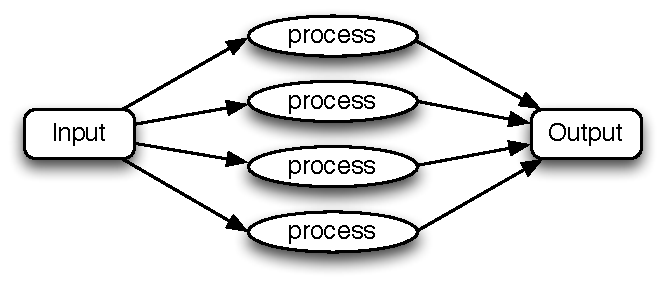
\includegraphics[width=3in]{figs/overview}
  \caption{A high-level architecture of our approach}
  \label{fig:overview}
\end{figure}

% You may need to move this \begin{figure} ... \end{figure} block around
% in the document to place it in a logical spot in the paper. In
% general, get the figure on the same page as the prose that refers to
% it.


\section{Design}
\label{sec:design}

Protocol/Architecture/Design/\ldots

\section{Evaluation}
\label{sec:eval}

\subsection{Characterizing Data Set}

Docker Hub currently host around 400,000 images. To perform experiments with DockerGate, it was required to limit our dataset to test and evaluate. Docker Hub hosts two types of images viz. Official images and Community Images. Official images are maintained by official owners of applications and community images are maintained by users and community members which contain some customized applications developed on top of official images.

To characterize the images we used the Dockerfiles of each image. Dockerfile for Official Images were obtained from the links consolidated in Docker’s Official Library repository[9]. While Dockerfile(s) for community images were obtained using a web scraper. We used ScraPy~\cite{scrapy}, a web scraping framework, to scrape Docker Hub for image names. Using random English dictionary words as search keywords, we were able to get about 96,000 Docker image names. Because of limitations in resources, we randomly sampled 110 Docker image names from those 96,000 names. We conduct our further experiments on this sample of 110 Docker images.

We analyzed these Dockerfiles to determine the nature of docker images. We first identified the base image of the docker image, which can be obtained from Dockerfile’s first line starting with keyword FROM. We analyzed the official images and community images separately. The result of this analysis can be found in Table~\ref{topbaseimages}.

As can be observed from Table~\ref{topbaseimages}, out of total 536 Dockerfiles, 118 images have Openjdk base images. Since Docker images can be derived from each other, we investigated the base images for OpenJDK and buildpack-deps. It was found that all these images were based on either Ubuntu, Alpine or Debian images as their most lowest level base image. The majority of the images were based on Ubuntu and Debian. A complete list of the distribution of images can found in the Appendix \ref{sec:appendix}.

Further we analyzed Dockerfiles of the community images obtained using web scraper. We randomly selected 400 images from the set and checked for the base image. It was observed that about 250 images had a base image of Ubuntu and Debian. While  about 100 images were based on Alpine, the rest of them were distributed equally among Fedora, CentOS and Scratch(Not based on any prior Docker Image).


Since the Ubuntu and Debian images was more popular in usage for developing the custom docker images, we have considered only Ubuntu or Debian based images for the analysis and testing of DockerGate.

\begin{table}
\centering
\resizebox{\columnwidth}{!}{%
\begin{tabular}{|l|l|}
\hline
\textbf{Base Image} & \textbf{Number of docker images} \\ \hline
openjdk & \multicolumn{1}{c|}{118} \\ \hline
buildpack-deps & \multicolumn{1}{c|}{79} \\ \hline
debian & \multicolumn{1}{c|}{78} \\ \hline
alpine & \multicolumn{1}{c|}{73} \\ \hline
scratch & \multicolumn{1}{c|}{49} \\ \hline
php & \multicolumn{1}{c|}{42} \\ \hline
python & \multicolumn{1}{c|}{15} \\ \hline
microsoft/windowsservercore & \multicolumn{1}{c|}{12} \\ \hline
microsoft/nanoserver & \multicolumn{1}{c|}{9} \\ \hline
ubuntu & \multicolumn{1}{c|}{9} \\ \hline
\end{tabular}
}
\caption{Top 10 base images used in building a Docker Image}
\label{topbaseimages}
\end{table}
We then analyzed the average file composition of a Docker Image. Out of a random sample of 110 Docker images, we analyzed the file types for all the executable code in each. As shown in Table ~\ref{filecompose}, it was found that ELF files and Python scripts made up most of the executable code in an average Docker Image. So, we decided to analyze ELF files to generate the Seccomp Policies. This was also supported by the fact that Python files were linked to ELF shared-object libraries. So by analyzing ELF files, we could provide some coverage for Python executable code as well.

\begin{table}
\centering
\resizebox{\columnwidth}{!}{%
\begin{tabular}{|l|l|}
\hline
\textbf{Container Status} & \textbf{Number of docker images} \\ \hline
Successful Execution & \multicolumn{1}{c|}{80} \\ \hline
Failed Execution & \multicolumn{1}{c|}{30} \\ \hline
\textbf{Total} & \multicolumn{1}{c|}{\textbf{110}} \\ \hline
\end{tabular}
}
\caption{Container status after loading them with DockerGate generated Seccomp policy}
\label{tab:seccompresults}
\end{table}

\begin{table}[b]
\centering
\begin{tabular}{|l|c|}
\hline
\textbf{File Type} & \textbf{No. of Files (in percentage)} \\ \hline
ELF Files          & 28                                    \\ \hline
Python Scripts     & 35                                    \\ \hline
Shell Scripts      & 14                                    \\ \hline
Others             & 23                                    \\ \hline
\end{tabular}
\caption{Average File Composition for Executable code of a Docker Image}
\label{filecompose}
\end{table}



%\begin{figure}
%    \begin{tikzpicture}
%        \begin{axis}[
%            symbolic x coords={ELF, Python, Shell, Other},
%            xtick=data
%          ]
%            \addplot[ybar,fill=blue] coordinates {
%                (ELF,   28)
%                (Python,  35)
%                (Shell,   14)
%                (Other,   1.1)
%            };
%        \end{axis}
%    \end{tikzpicture}
%    \caption{Average Composition for Executable code of a Docker Image}
%    \label{filecompose}
%\end{figure}


\subsection{DockerGate Policy Evaluation}

%We use DockerGate by providing the name of a docker image as input to DockerGate, further it performs the analysis and updates the global database of system calls if required and generates a seccomp  policy. 

% Write Table Legend Here
% Replace following terms as in tables

After issuing a docker run command, the launched container can be in three possible states. 
\begin{itemize}
\item \textbf{Up} - the container is up and live, applications within the container are being executed as expected.
\item \textbf{Created} - in this state it creates a writable container layer but doesn’t start the container execution.
\item \textbf{Exit} - the container is destroyed and all the resources are freed. Depending on the exit code, it determines if container was gracefully destroyed or with some error in the application. Exit code of 0 indicates a graceful exit, while any other code indicates an erroneous exit from container
\end{itemize}

We determine the generated Seccomp policy for docker images to be successful by applying the generated policy and attempting to create and execute a simple container. If the status of the container is Up or if it exits with exit code 0, we assume that the container was created successfully and was able to execute the entry-point application within the container. We also verified the success of a container by executing the basic commands within the container. If the result of these commands was successful then we considered the container might function normally. The commands that we tested were \textit{uname, mkdir, /bin/sh \& echo}. If the container exited with a non-zero code or entry point failed to execute or appeared to hang-up, we considered it a failure in the Seccomp policy.
% Replace this with actual images results
From a set of Ubuntu based docker images, we executed DockerGate on randomly selected 110 community images. The images contained applications ranging from simple binary files to complete Databases and Web Servers. 





From the Table \ref{tab:seccompresults} we can see that 80 out of 110 containers exited in successful state. While 30 of them ended in failure. Further we analyzed the failed images, in which we observed 17 images crashed during execution i.e. they exited the container with status greater than 0 \{e.g. 1, 139, 159\}. The remaining 13 images out of 30 failed images ended up in \textbf{Created} state. The Created state indicates the seccomp policy was successful in initiating the containers but not successful in execution. The reason  we speculate is that the container didn't had any executable binaries but relied on script based languages or other native languages like JavaScript, Python or Java.   

The Failed images also included 3 images which had failed to execute because the seccomp policy generated didn't include some of the system calls. This caused the container to exit erroneously.

To determine which system calls were used during the execution of the container we used a tool called SystemTap~\cite{systemtap}. We developed a custom SystemTap script which would print the system calls being called during the execution of the container. The reason why we could trust System Tap in this case, as compared to strace is that, when a system tap script is executed, a custom Linux kernel module is created and inserted into the kernel. Based on the probe events defined in the script, when any such event is triggered corresponding action is executed in the kernel space. This allowed us to identify exactly which system calls had been used by any command, which in this case, was the Docker container. 

We spawned the Docker container for same 110 images used above and obtained the system calls called during the process. In the 110 images above, we found that an average of 118 system calls are actually required for spawning and initiating the start up process within the container.

Thus from the above experiments conducted, we can derive a lower bound on the number of system calls a docker image with base Ubuntu image can have. With an average of \textbf{minimum 118 system calls} a basic Ubuntu image can be  successfully executed, while our \textbf{DockerGate framework generates seccomp policy with average number of system calls equal to 213}. 

The current default seccomp policy includes about over 300 system calls to be allowed to be executed, which exposes a large attack surface for the host kernel. Based on the result of experiments conducted, the default policy can be reduced to 213 system calls identified above and reduce the attack surface of the host kernel. 

During the evaluation of the images we observed that 17 system calls were required to create a container from its image. Hence, these system calls were included by default when generating the policies. A full list of these system calls can be found in Appendix.
\section{Discussion}
\label{sec:discussion}
Using static analysis to develop system wide policies has its limitations. The correctness of the policies depends upon the code coverage of the system. While DockerGate does analyze most of the ELF executables and shared objects, executable code like Java JAR files still remains out of scope for DockerGate. Since many images do use Java, this poses to be a threat to validity as the system calls these files make are left out of the policy.

In our ELF shared-object analysis, we have tracked the contents of the EAX register till just before the system call. However, while we do handle the "mov" instruction recursively as explained in Section~\ref{sec:design}, there were some cases where the contents of EAX were being modified by other instructions such as XOR and ADD. Such examples were fewer in nature. But we had to log them as exceptions that DockerGate could not handle.

We have focused solely on static analysis in DockerGate because of the reasons cited in 
Section~\ref{sec:background}. We believe that if a technique could be found that could execute all possible branches of the executable code in a Docker container, dynamic analysis could be combined with DockerGate to provide tighter policies. Such work has been done Android Applications[cite] and could be expanded to Docker containers. While static analysis gives a complete overview of what system calls are required, the dynamic analysis could remove the system calls present in dead-code or code that can never be reached during the execution of the application in the Docker container.

DockerGate can also be extended to produce AppArmour~\cite{apparmor} profiles. AppArmour profiles can control the permissions the program in a container can have. These permissions range from read/write/execute abilities on certain files to network access. AppArmour and Seccomp profiles combined can further reduce the attack surface on the host kernel as an attacker would not be able to use an existing program outside the bounds defined by both the security modules.

\section{Related Work}
\label{sec:relwork}

After the introduction of the containers, many developers have focused on container hardening which uses the kernel capabilities and features to protect and secure the containers. Various approaches have been proposed earlier where different kernel features can be used to secure the container. One such approach, as proposed by Rastogi et al.~\cite{rastogi}, is to divide a container into simpler containers to have limited functionality with least privilege, while preserving the overall functionality of the Image.  

Provos ~\cite{provos2003improving} proposed \textit{Systrace} to facilitate process-specific policy generation based on how the processes invoked system calls. This was a Dynamic Analysis technique that monitored the behaviour of the processes. Policy generation has also been attempted with SELinux ~\cite{sniffen2006guided, harada2003access} and with Android Applications ~\cite{afonso2016going}. However, with Docker being a young technology, it hasn't gained much traction on research in academia. But there are many community developers who attempt to bring tools or solutions in various aspects of the Docker. Docker-Slim~\cite{dockerslim}, is a similar project which primarily depends on dynamic analysis of the Docker containers. However, as discussed earlier in this paper, it is difficult to perform dynamic analysis because of the varied number of applications running inside the container. On the contrary, the static analysis scans all eligible files and  identify all possible system calls made by the binaries executables present in the docker image. As seen in ~\cite{afonso2016going}, the code coverage by dynamic analysis despite having an automation framework ranges from 8-10\%.  

One more kernel feature that can be exploited for container hardening is AppArmor. LiCShield~\cite{mattetti} exploits this feature by generating rules for restricting the access of a docker container by monitoring the changes made by processes associated with container and convert it into Linux security module for AppArmor. The works of LiCShield was based on Docker 1.6 version which didn’t had the support of Seccomp and AppArmor profiles, but were required to depend on host operating system to implement AppArmor. LiCShield was required to be supported by the host operating system and Docker was not involved in any way. They monitored and controlled the processes forked by Docker daemon.


There have been proposals~\cite{dockerpolicymodules} related to shipping a SELinux policy along with the docker image, where SELinux features are enabled on the host machine, and the SELinux policy is applied to the docker containers executed from this image. But this proposal requires that all the host operating systems must have SElinux policy installed and enabled which is by default is disabled for most Linux based systems. According to the study by Raj et al~\cite{raj2016}, using the security features like AppArmor and SELinux policies built in Docker, the various stages of DevOps pipeline can be secured and based on suitable profiles can secure the stages and deployments. Their experiments claim to mitigate certain security risk vectors.

Rajagopalan et al~\cite{rajgopalan} proposed Authenticated System Calls which performed static analysis on executable binaries to replace the system calls with custom system calls. But this required modification in the host kernel which may affect the integrity of host kernel.
\section{Conclusion}
\label{sec:conc}

Conclusions (don't summarize your work here. That's what the abstract
was for. Instead provide some philosophical ruminations of your work and
future possibilities, i.e., conclusions that you have arrived at as a
result of your work.)


\bibliographystyle{abbrv}
\bibliography{main}

\end{document}


